\pagestyle{plain}
\chapter{Prologue} % single size step larger than text font
\renewcommand{\thetable}{\arabic{chapter}.\arabic{table}}  
\renewcommand{\thefigure}{\arabic{chapter}.\arabic{figure}} 

This is the introduction chapter, use it to introduce the audience to what this Thesis/Dissertation represents. Maybe your work is biology related and deals with proteins. Good graphics help assist with the introduction, see Figures \ref{fig:ala} and \ref{fig:ASN-ALA-CYS}. You might also want to mention your related publications.
%This research The sequence of amino acids that comprise a protein determines the shape and function, or more specifically, how the protein interacts with other proteins. Regardless of reference to the catalytic power of a protein, or the selectivity a certain protein has for interacting with another \citep{Garrett2010,Ma2011,AbdoolKarim2010}, the end result is a protein-protein interaction. 

\begin{figure}[h!]
\centering
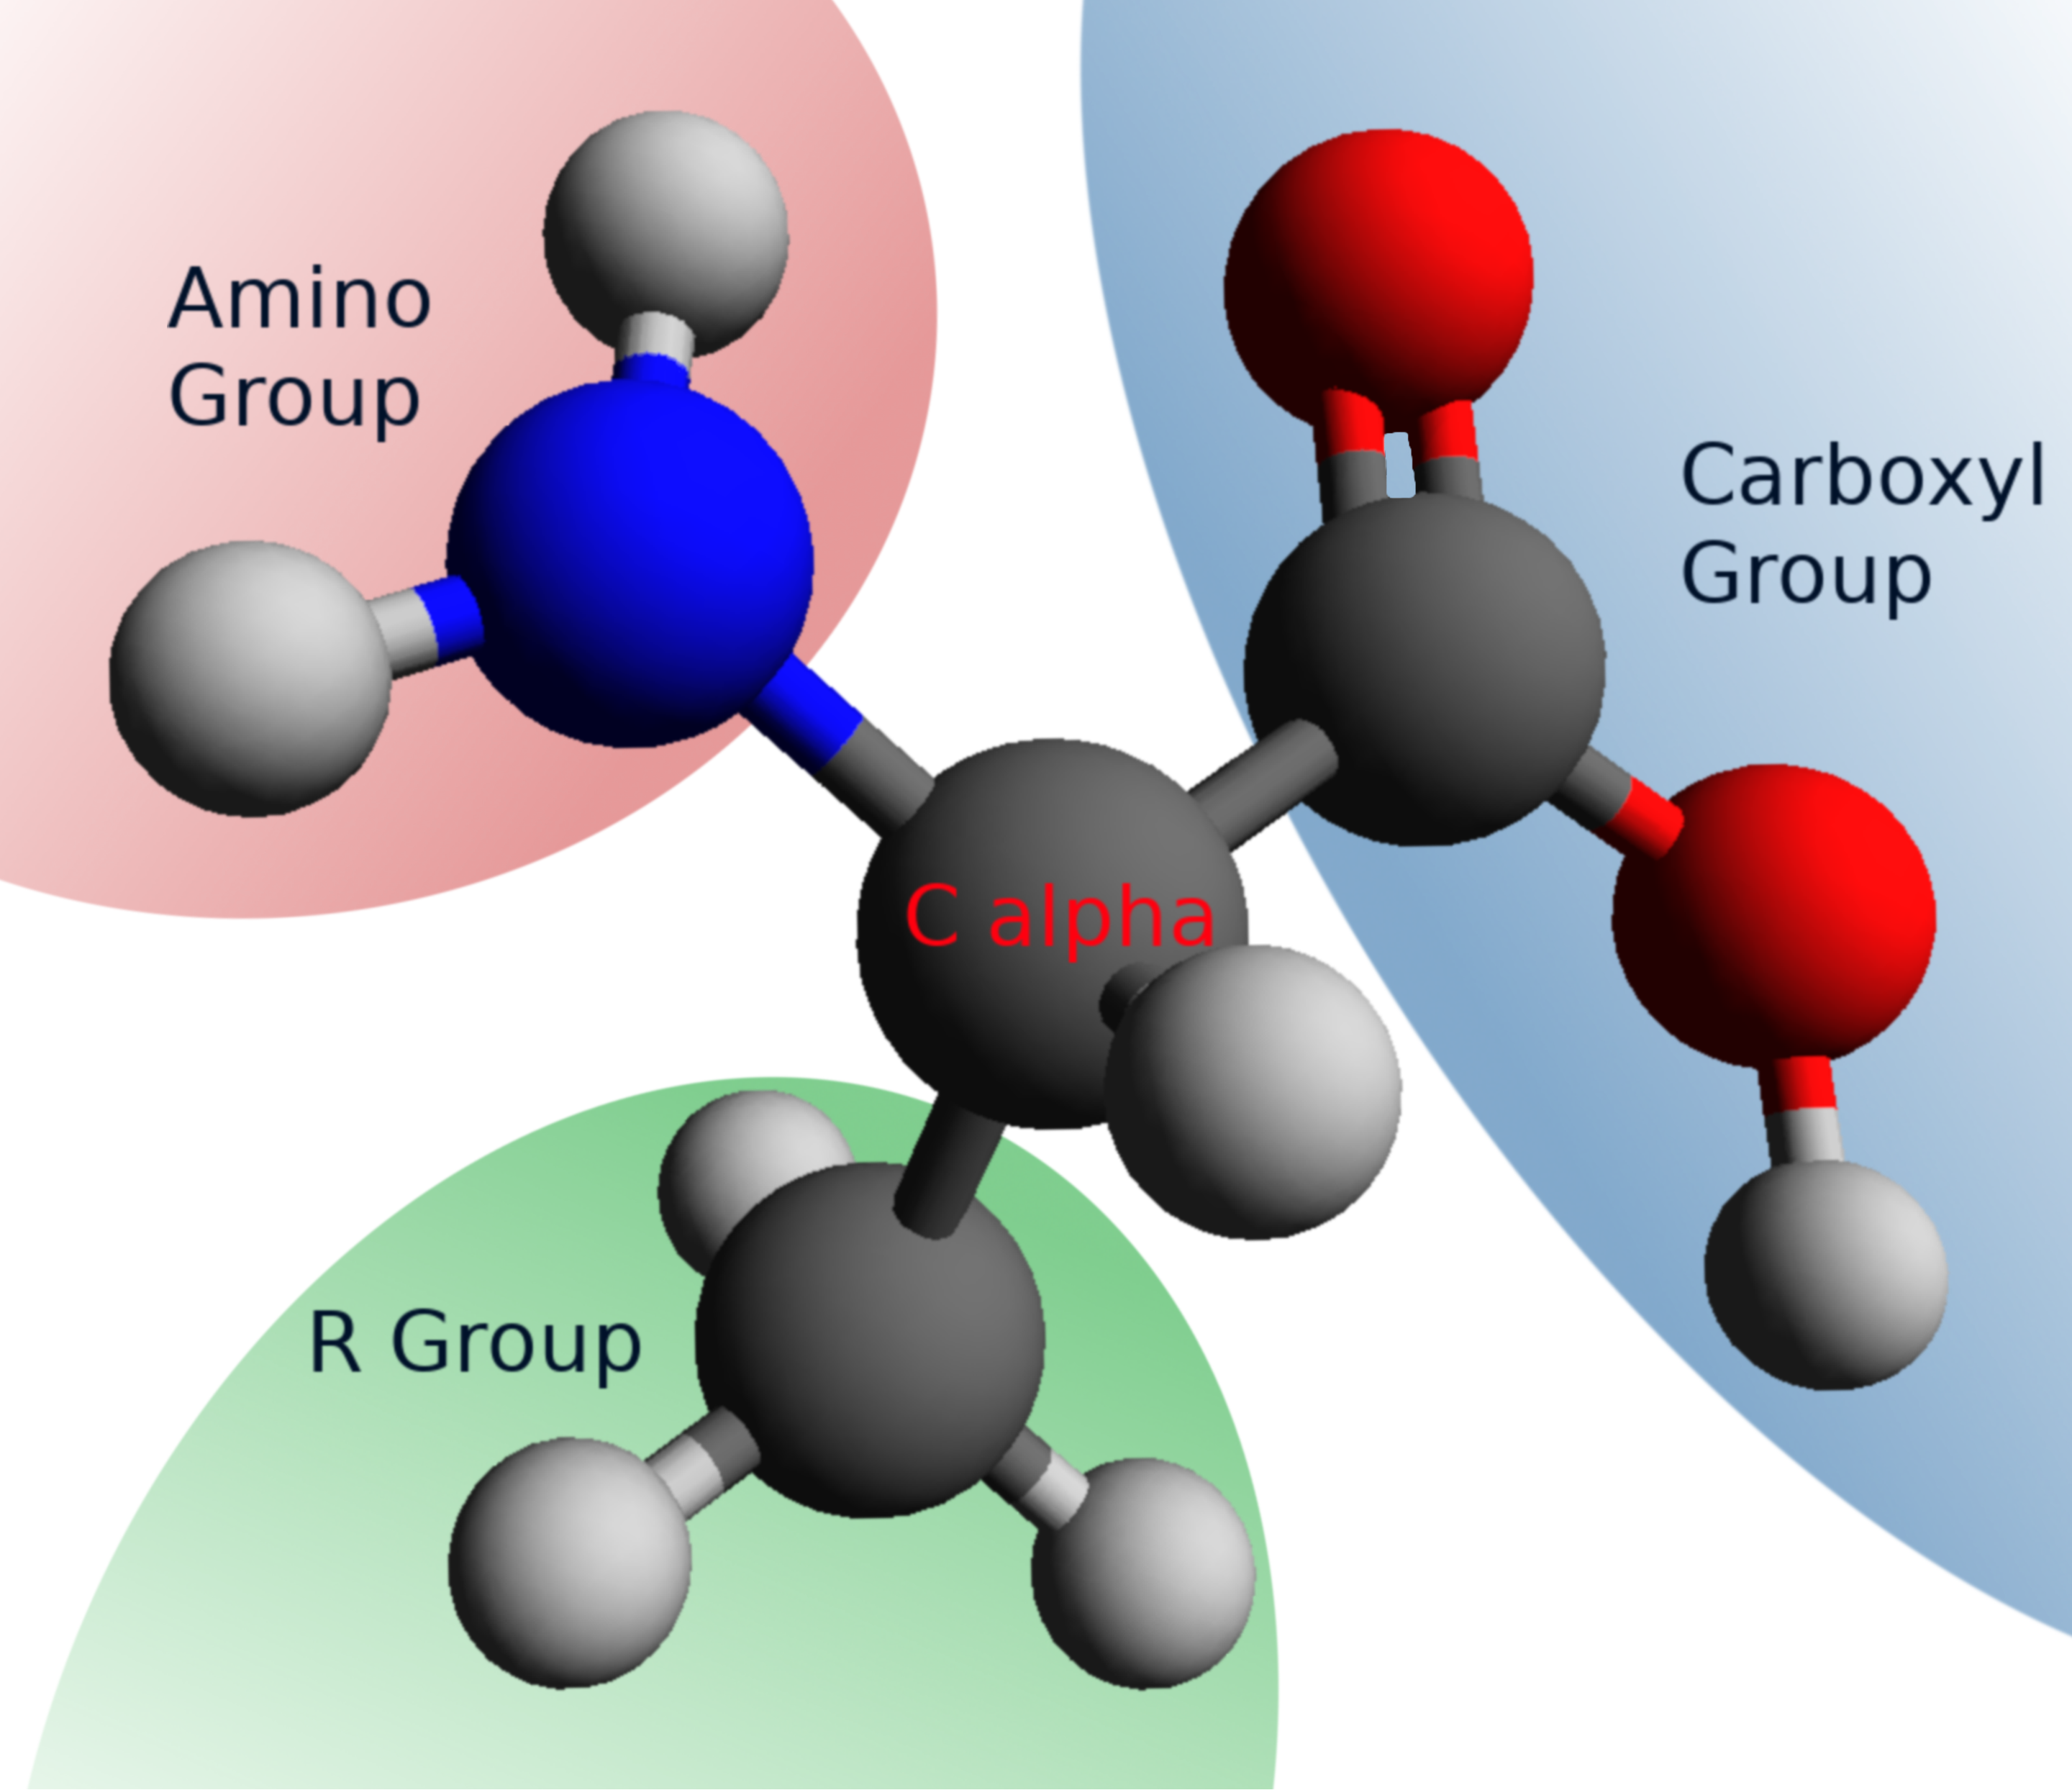
\includegraphics[width=0.7\linewidth]{images/ALA2}
\caption{The amino acid Alanine showing the amino group (red shading) bound to the alpha carbon $CH$ (center) that is bound to the carboxyl group (blue shading). The R group (green shading)  for Alanine is $CH_3$. Carbon is depicted as dark gray, hydrogen is light gray, oxygen is red and nitrogen is blue. Amino acid produced by Avogadro \citep{Hanwell2012}.}
\label{fig:ala}
\end{figure}

\begin{figure}[h!]
\centering
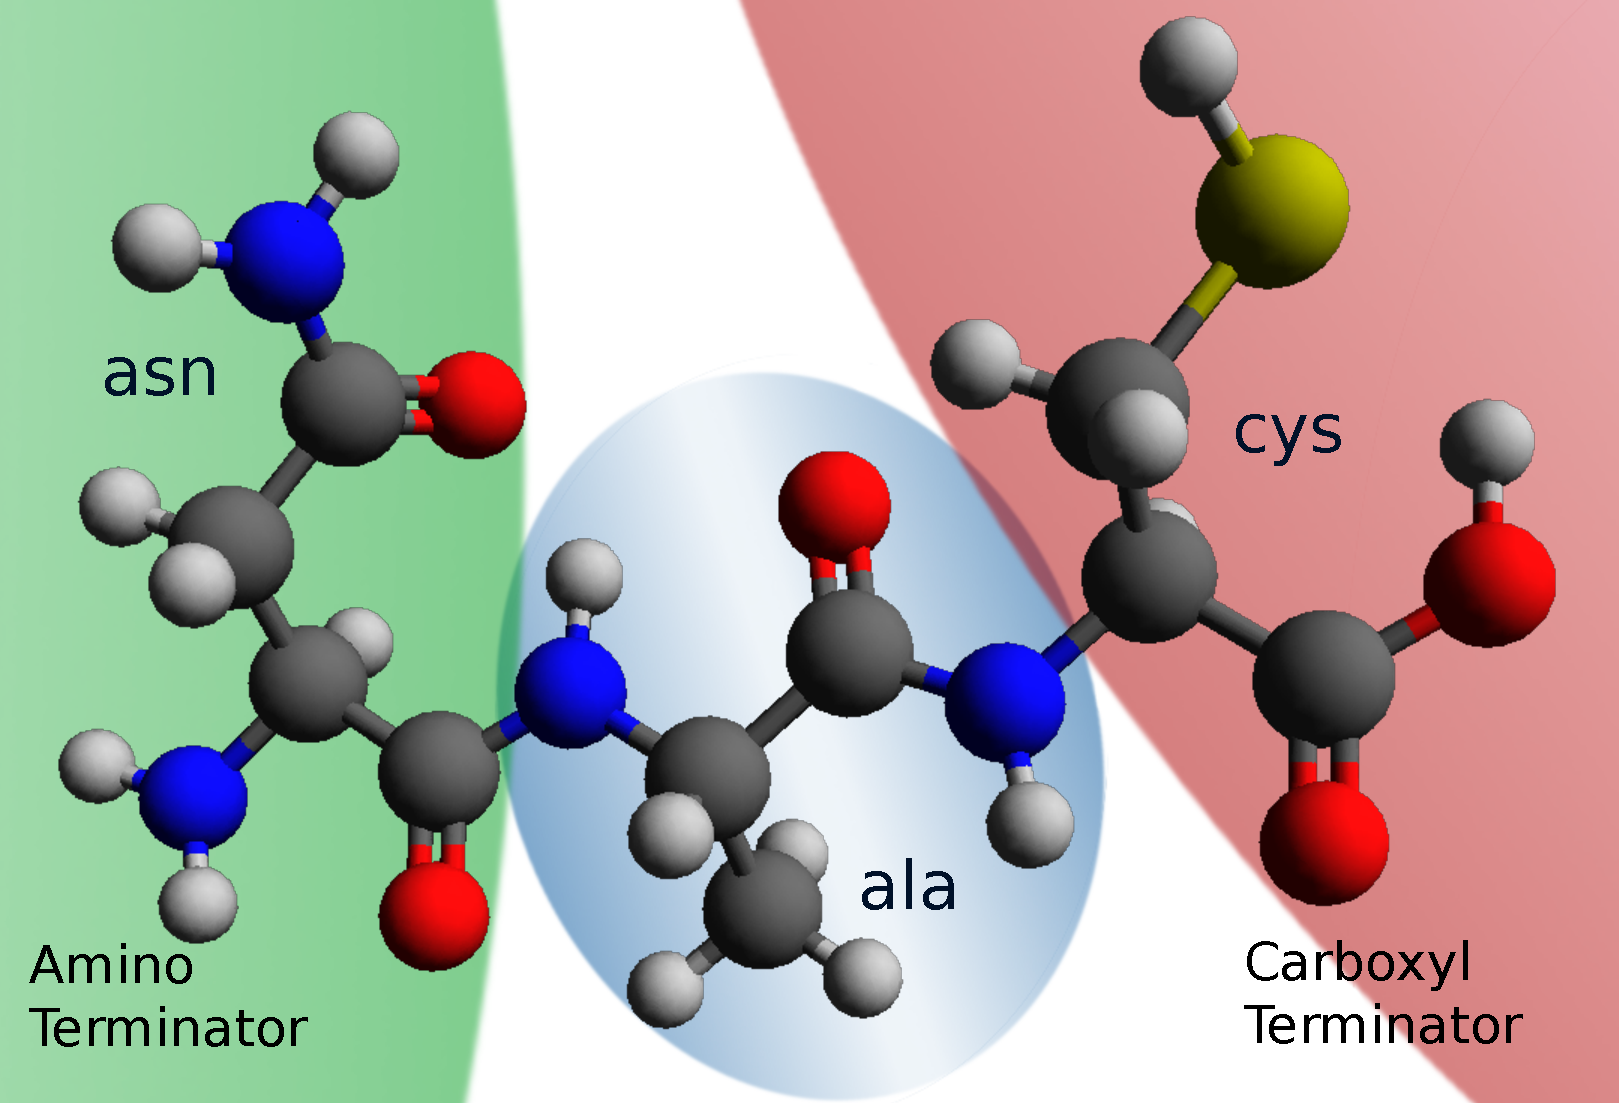
\includegraphics[width=0.7\linewidth]{images/ASN-ALA-CYS}
\caption{A simple protein chain with shading to distinguish each amino acid: Asparagine (green), Alanine (blue), and Cysteine (red). The amino terminal is to the left and the carboxyl terminal is to the right. Carbon is depicted as dark gray, hydrogen is light gray, oxygen is red, sulfur is yellow and nitrogen is blue. Protein chain produced by Avagadro \citep{Hanwell2012}.}
\label{fig:ASN-ALA-CYS}
\end{figure}


\noindent The following are related publications:

%\SingleSpacing
\begin{list}{}{}
	\item “Still Working on this Awesome Paper” (In preparation)

	\item Me, and You. “A Paper I Submitted and Currently Have a Preprint on BioRxiv.” BioRxiv, Cold Spring Harbor Laboratory, June 2020, the doc id and url. (Submitted for publication)

	\item Me, You, and Another ...

\end{list}
%\DoubleSpacing

